\documentclass[12pt,a4paper,reqno]{amsart}
\usepackage{format}
\geometry{margin=0.5in} % Smaller margins for more work.
\setlist[enumerate,1]{label=(\alph*)}
\usepackage{hyperref}   % Enable embedded hyperlinks
\usepackage{wrapfig}

\usepackage[style=numeric, citestyle=numeric]{biblatex}
\addbibresource{references.bib}

\let\bm\undefined
\newcommand{\bm}[1]{\mathbf{#1}}
\let\x\undefined
\newcommand{\x}{\bm{x}}
\let\y\undefined
\newcommand{\y}{\bm{y}}
\let\z\undefined
\newcommand{\z}{\bm{z}}
\let\n\undefined
\newcommand{\n}{\bm{n}}

\let\Cin\undefined
\newcommand{\Cin}{C_{\mathrm{in}}}
\let\Cout\undefined
\newcommand{\Cout}{C_{\mathrm{out}}}

\let\G\undefined
\newcommand{\G}{\mathcal{G}}
\let\V\undefined
\newcommand{\V}{\mathcal{V}}
\let\E\undefined
\newcommand{\E}{\mathcal{E}}
\let\L\undefined
\newcommand{\L}{\mathcal{L}}
\let\F\undefined
\newcommand{\F}{\mathcal{F}}

\newcommand{\soa}{state-of-the-art}

\title{Deep Graph Convolutional Networks for Image Denoising}
\author{Nikola Janju\v{s}evi\'{c}, \texttt{npj226}}
\date{\today}

\begin{document}

\begin{abstract}
This report walks through the implementation of the Graph Convolutional
Denosising Network (GDCN) as detailed in \cite{ValsesiaICIP19}. The mentioned
work proposes a novel image denoising deep neural-network that dynamically
builds K-regular graphs in feature space to exploit non-local self-similarity of
the underlying signal. It is an addtion to the ever growing body of work on
non-local methods in signal processing, and has achieved state of the
art-performance on popular image denoising benchmarks (both real and synthetic). 
Background is given to understand the mechanics of the algorithm's novelty.
Some additional insights are given in the implementation of the method.
Small scale experiments are done to verify the benifit of the graph signal
processing. 
\end{abstract}

\maketitle

\section{Introduction}
Denoising is perhaps the most fundamental problem in signal processing. Although
it has recieved decades, if not centuries, of attention, it remains a hot
topic in today's literature as a proving ground for new ideas and algorithms.
This is largely becuase the denoising problem presents one of the simplest
observation model, $\y = \bm{A}\x + \n$, where $\n$ is sample of noise following
some distribution, and the observation operator $\bm{A}$ (in this case) is the
identity. We refer to the problem of obtaining the signal $\x$ from observation
$\y$ as an \textit{inverse problem}, which in image-processing includes
densoising, deblurring, super-resoluiton, and more. Thus, for the most part, any
inverse-problem solving algorithm must also be a good denoiser. To further
simplify the problem, as will be done in this implementation, we often look at
evaluating our algorithms on synthetic white Gaussian noise, where $\n \sim
\N(0,\sigma_n^2)$. Though additive Gaussian white noise (AWGN) is by no means a
sophisticated model for real world noise (especially camera noise), it is a
convienient benchmark which is widespread in the literature. See
\cite{real_denoising_refs} for extending modern denoising algorithms to
real-world noise models. \\

In this report we present an implementation of a \soa deep-learning based
denoising method \cite{ValsesiaICIP19} for images. Recently, learning based
algorithms have come to dominate not only computer-vision tasks but also
image-processing tasks such as denoising. This leap in performance was generated
by the advent (and later efficient implementation) of convolutional neural
networks (CNNs). Much of the CNNs success can be attributed to its bias towards
exploiting local information (via convoluiton). Further gains in the performanc
of deep-learning methods are increasingly being sought by explointing both local
and non-local information of the input signal. These ``non-local" methods come
in many different flavors, mainly differing in their definitions of non-local
neighbors and aggregation operators. The fruits of non-local methods are
illustrated in Figure \ref{fig:fruit}, where the use of graph-convolutions in the
implemented GCDN network has changed the uniform, radially growing receptive
field, to a content-dependent adaptive one. \\

The remainder of this report is outlined as follows. In Section
\ref{sec:background} we first introduce the concepts and noation necessary for
understanding the graph signal processing used in the GCDN
\cite{ValsesiaICIP19}. We then go over the differences between the non-local
operations of GCDN and other popular (learned) non-local methods. In Section
\ref{sec:implementation} we detail our implemented GCDN. Finally, in Section
\ref{sec:experiments} we show some experiments from the implementation.

% -----------------------------------------------------------------------------
% -----------------------------------------------------------------------------
% -----------------------------------------------------------------------------

\section{Background and Related Works} \label{sec:background}
\subsection{Convoluitons on Graphs}
The emerging field of graph signal processing (GSP) seeks to extend classical
signal processing knowledge and technqniques to signals defined on irregular
domains (non-uniform grids, etc.). In doing so a more general formulation of
common operations, such as convolution, must be obtained, which may also bring
benefits to signal processing on regular domains, such as images. Lets first
introduce some notation: \\

\textbf{Notation}: Consider a multi-channel signal (ex. RGB image) with 
$C$ channels and $N$ pixels, $\x \in \R^{CN}$. 
\begin{itemize}
\item $\x[i] \in \R^C$, feature vector corresponding to pixel $i$.  \\
\item $\x^k \in \R^N$, channel $k$ of $\x$.  \\
\item $\G(\V,\E)$, directed graph with vertices $\V$ and edges $\E$. \\
\item $\V$, set of vertices (pixels). Caridinality $\abs{\V} = N$. \\
\item $\E$, set of edges. $\E \subseteq \V \times \V$. \\
\item $\N(i) = \{j | (i,j) \in \E \}$, set of neighbors of vertex $i$. \\
\item $\L: \E \rightarrow \R^M$, label mapping.
\item $\L[i,j] \in \R^M$, label for the edge connecting vertex $j$ to $i$.
\end{itemize}

\subsubsection{Frequency vs. Spatial Domain Definitions of Graph Convoluiton}
Convolution is a staple of signal processing as it defines any linear
shift-invariant (LSI) system. The operator is diagonalized by the Fourier basis
and as such can equivalently characterized in both the frequency and spatial
domain. For extending the concept of convolutions to signals defined on graphs, 
several formulations have been proposed. A graph-laplacian matrix based on the
graph's adjacency matrix can be used to yeild a spectral decompostion. However,
the formation and application of this operator can be expensive, which is
undesirable for situations with dynamically changing graphs. An alternative
approach is to define graph convolution in the spatial domain as an agregation
over neighboring vertices. This more general formulation loses the nice
properties of spectral theory gains simplicity, flexiblity, and speed.

\subsubsection{Edge Conditioned Convolutions}
The GCDN architecture uses the graph convolution formulation from
\cite{Simonovsky2017ecc} known as edge conditioned convolution (ECC). Suppose we
have a multi-channel signal with $C_in$ channels and $N$ pixels, $\x \in
\R^{\Cin N}$ and an associated graph with vertices, edges, and edge-labels,
$\G(\V,\E,\L)$, $\abs{\V}=N$. Further, consider the mapping $\F:\R^M \rightarrow
\R^{\Cout \times \Cin}$. We define the edge conditioned convolution of $\x$ by
$\F$ as 
\begin{align}
\y[i] &= \sum_{j \in \N(i)} \F(\L[i,j])x[j], \quad i=1,\dots,N \\
      &= \sum_{j \in \N(i)} \bm{H}_{i,j}x[j] \in \R^{\Cout}. \nonumber
\end{align}
We call $\F$ the label-operator mapping and $\bm{H}_{i,j}$ the
(edge-conditioned) feature operator from vertex $j$ to $i$. ECC is performing a
node-aggregation in which the contribution of an
input node in the neighborhood is determined by an associated label-generated
operator. \\

In the 1D case ($\Cin = \Cout = 1$), we note that ECC can reduce to the
linear convolution, $\y = \bm{h} \ast \x$. First, we define the graph such that only
immediate neighbors are connected, and edge-labels as
$\L[i,j] = \delta[i-j]$, where $\delta$ is the discrete impulse function. Then, 
define the label-operator mapping as $\F(x) = \bm{h}^\top \x$. Together, we
arrive at $\y[i] = \sum_{j=-M/2}^{M/2-1} \bm{h}[i-j]\x[j]$, the famed discrete
convolution formula.

%\subsection{Non-local methods for image restoration}

% -----------------------------------------------------------------------------
% -----------------------------------------------------------------------------
% -----------------------------------------------------------------------------

\section{Implemented Denoiser} \label{sec:implementation}
\subsubsection{Overview}
An overview of the GCDN architecture is presented in Figure \ref{fig:arch}.
The network employs a residual learning strategy by adding the input signal to
the output of the very last stage. The main path consists of a ``multi-scale"
preprocessing block (3 parallel paths processing the input with different filter
sizes, $3,5,7$). After the preprocessing stage, the signal goes through several
``LPF" blocks which themselves involve a residual connection between input and
output. Another residual connection in the main path is given from the
preprocessing block, through a ``HPF" block, and connected to the output of each
''LPF" block. The heavy use of residual connections (and leaky-ReLUs) is
reportedly for the purpose of mitigating vanishing gradients. Furthermore, the
architcture's inspiration is said to derive from an algebraic manipulation of an
unrolled proximal-gradient descent algorithm with a graph-laplacian regularizer
\cite{ValsesiaICIP19}.  

\begin{figure}[t]
\centering
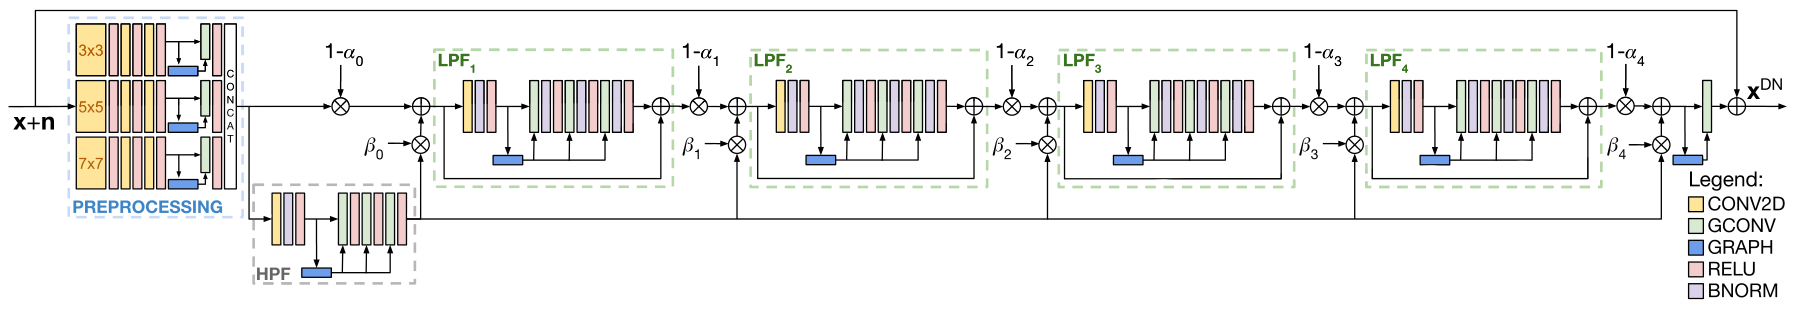
\includegraphics[width=\textwidth]{imgs/gcdn_arch.png}
\caption{Graph Convolutional Densoising Network \cite{ValsesiaICIP19}
architecture. All ReLU blocks are leakly-ReLUs with negative slope of $0.2$.
$\alpha_i,\beta_i$ are scalars learned for each iteration.}
\label{fig:arch}
\end{figure}

The defining feature of the network resides within each of these blocks:
the graph conovlutional layer. These layers perform edge-conditioned
convolutions with the input signal provided an input graph. The graphs are
formed as $K$-regular graphs via a $K$ nearest neighbors (KNN) algorithm in the
feature domain. The edge-labels of said graph are defined as the vector from
node $j$ to $i$, $\L[i,j] = \z[j] - \z[i]$, where $\z$ is an input latent signal.
As the computation of the KNN graph can be computationally expensive, the same
graph is reused through a single network block -- although the labels still
change within blocks.

\subsection{Graph Convoluitonal Layer}
The graph convolutional layer is defined as the average of a (local)
convolutional operation and a non-local graph convolution operation, as
represented pictorially in Figure \ref{fig:gclayer}.

\begin{figure}
\centering
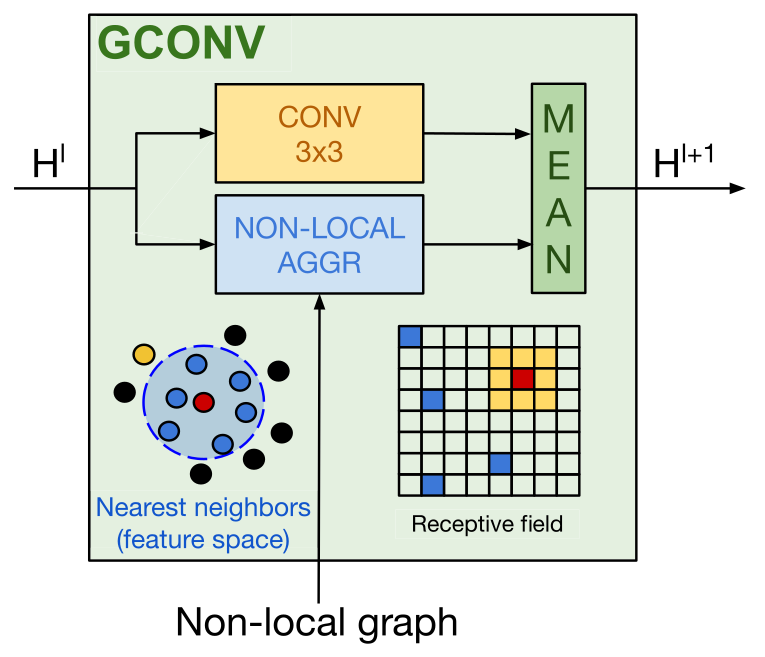
\includegraphics[width=.35\textwidth]{imgs/nlagg.png}
\caption{Graph convoluitonal layer \cite{ValsesiaICIP19}. A local 2D convolution
is averaged with a non-local edge-conditioned convolution given an input graph.
The input graph explicitly excludes neighbors within each pixels local area,
defined by the size of the local convoluiton's filters. }
\label{fig:gclayer}
\end{figure}

The authors of GCDN \cite{ValsesiaICIP19} employ an augmented definition of ECC,
\begin{align}
z[i]^{(\ell+1),\mathrm{NL}} &= \sum_{j \in \N(i)} \gamma[i,j]
\F^{(\ell)}_{\bm{w}^{(\ell)}}(\L[i,j])\z[j]^{(\ell)} \\
&= \sum_{j \in \N(i)} \gamma[i,j] \Theta_{i,j}\z[j]^{(\ell)}. 
\end{align}

This formulation is consistent with our previous formulation up to the label
dependent scale factor, 
$$
\gamma[i,j] = \exp\left( - \norm{L[i,j]}^2 / \delta \right).
$$
In fact, this formulation is exactly equivalent to the original ECC definition
except that we explicitly model a dependence of proximity in the feature domain
(label-domain). The graph convolutional layer is then defined as 
\begin{equation}
\z^{(\ell+1)} = \frac{\z^{(\ell+1),\mathrm{L}}+ \z^{(\ell+1),\mathrm{NL}}}{2} +
\bm{b}^{(\ell)}.
\end{equation}

The label-operator mapping $\F$ is implemented by a 2-layer multi-layer
perceptron (MLP) for each graph-conv layer, with some caveats for memory
consideration and overparameterization, as described in the following section. 

\subsection{Lightweight ECC}
Consider a signal inside the network of $M$ channels and $N$ pixels, which is to
be transformed into another signal of $M$ channels. In the graph convoltional
layer, we propose that for every pixel, its $K$ neighbors each have their own
feature-operator of size $M\times M$. For processing relatively small image of size $N = 256$,
with feature vectors $M=128$ and $K=8$ nearest neighbors, this single layer
would require 64Gb to store just the associated feature-operators. Further more,
the feature-operators are generated by a single feature vector, and thus largely
over-parameterized. The GCDN network thus employs circulant approximations of
dense layers in its label-operator mappings $\F$, and low-rank
feature-operator matrices to tackle the over parameterization and memory
problems respectively.  \\

\textbf{Circulant approximation of dense layers}: The circulant approximation of
dense matrices is applied in both layers of the MLPs that define $\F$. It can be
viewed as replacing a matrix multiplication with a 1D (valid) convolution where
the filters are of the size of the input and the input is padded with $m$ values
(from a circular shift). We then say that $\F$ is approximated with
$m$-circulant matrices. Clearly, this approximation is able to reduce the number
of parameters in $\F$ by a factor of $m$.  \\

\textbf{Low-rank edge conditioned convolution}: We can further reduce the
computational and memory burdens of ECC by explicitly factorizing the
feature-operators $\Theta[i,j]$ as a sum of $r$ outer-products, yeilding an
operator of at most rank $r$. This is implemented by having three parallel
branches in the second layer of $\F$ MLP that produce factors, $\Theta^L,
\kappa, \Theta^R$ to create an SVD-like factorization: $\Theta = \Theta^L
\diag(\kappa) \Theta^R$.

Further care is taken to insure proper initialization of the label-operator
mapping for smoother training. 

\section{Experiments} \label{sec:experiments}
The Pytorch implementation of GCDN is available
online\footnote{\url{github.com/nikopj/DGCN}}.

\subsection{Training Setup}
The network was trained on patches of size $32\times 32$ from the Berkley
Segmentation Dataset, BSD400 \cite{bsd}, and evaluated on the associated test
set, BSD68. A batch size of 4 is used and the networks are trained for roughly
$40k$ iterations -- 20\% of the total training time reported in the original
paper. Despite this, training still took 36 hours on two GPUs for each network.
Other implementation details, such as rank and circulant approximation, match
that of the original paper. During training, nearest neighbor computations are
taken over the whole patch. During inference however, a sliding window of
$32\times 32$ is used to compute the KNN for each pixel. This method of
inference allows the receptive field of the network to adaptive in fantastic
ways across the input images. 

\subsection{Ablation Study}
- width of network and num. nearest neighbors
\subsection{Adaptive Receptive Field}

\section{Discussion}
\section{Conclusion}

\printbibliography


\end{document}
